\documentclass[prb,aps,twocolumn,floatfix,amsmath,amssymb,superscriptaddress,tightenlines]{revtex4}
\usepackage{graphicx}
\usepackage{epstopdf}
\usepackage{amsfonts}
\usepackage{bm}
\usepackage{color}
\usepackage{ulem}
\begin{document}

\section{Loop algorithm with ratio weighting}

We present a modification to the recently proposed algorithm using loop updates with quantum Monte Carlo in the valence bond basis.  This improvement aids in the measurement of the Renyi entanglement entropies.

%{\it The {\bf ?topology?} of the loop-operator list is modified.
%Differences:  links are changed across boundary between system copies, measurements values must be multiplied by $\langle Swap_x \rangle$ to get the value unmodified by the weight.}

\subsection{Valence bond quantum Monte Carlo}

Quantum Monte Carlo in the valence bond basis (VB QMC) is a ground state projection technique which, for the given Hamiltonian, yeilds a state proportional to the ground state wavefunction by applying a high power of that Hamiltonian to a  trial state, $\lvert \psi \rangle = \sum_i c_i \lvert i \rangle$,
\begin{eqnarray}
	\lvert 0 \rangle \propto \mathcal{H}^m \lvert \psi \rangle &=& \sum_{i=0} E_i^m c_i\lvert i \rangle  \\
	&=& E_0^m \left[ c_0 \lvert 0 \rangle + \sum_{i=1} \left(\frac{E_i}{E_0}\right) ^m c_i\lvert i \rangle \right] \label{gsproj},
\end{eqnarray}
where all but the first term of \eqref{gsproj} vanishes as $m \rightarrow \infty$ when $E_0$ is the energy with the largest magnitude.

In the case of the Heisenberg model, the Hamiltonian is modified by a constant shift and rewritten in terms of {\it bond operators} $H_{ij}$ which act on nearest-neighbour pairs of sites,
\begin{equation}
	 \mathcal{H} = \sum_{\langle i,j \rangle} \left({\bf S}_i \cdot {\bf S}_j - \tfrac{1}{4}\right) =  -\sum_{\langle i,j \rangle} H_{ij}.
\end{equation}
This allows us to sample terms in the ground state wavefunction by applying strings of $m$ bond operators to a trial state.

So far nothing we have done is basis specific, however, when these bond operators give a very simple results when applied to a valence bond state.  A bond operator acting on two sites already joined by a valence bond will not change the state.  In the other case, when the sites are not joined, the operator will join those sites and the resulting state will have a weight of $1/2$,
\begin{eqnarray}
	&&H_{ab}\lvert (a,b) \rangle=  \lvert (a,b) \rangle \label{bondop2}\\ 
	&&H_{ab}\lvert (a,d)(c,b) \rangle =  \tfrac{1}{2}\lvert (a,b)(c,d) \rangle, \label{bondop}
\end{eqnarray}
where $(a,b)$ represents a valence bond between sites $a$ and $b$.  
For non-bipartite lattices \eqref{bondop} could pick up a negative depending on the sublattice of the sites involved.  In this algorithm we only use valence bonds including one site from each sublattice.

MEASURING OBSERVABLES!!!!  

To simplify matters the list of $m$ bond operators can be rewritten as just one operator $P_i$ such that $\lvert 0 \rangle \propto \sum_i P_i \lvert \psi\rangle$.

From \eqref{bondop2} and \eqref{bondop}, we can generalize the action of $P_i$ on some state as $P_i \lvert \psi\rangle = W^i  \lvert \psi^i\rangle$, where $ \psi^i$ is the new state acquired from the application of the $m$ operators in $P_i$ and $W^i = 2^{-n_{\rm i}}$ contains all of the factors of 1/2 from applying operators which change the valence bond state as in \eqref{bondop}.

We can then measure observables...
\begin{eqnarray}
%\langle \mathcal{O}\rangle  &=& \frac{ \langle 0 \rvert \mathcal{O} \lvert 0 \rangle}{\langle 0 \lvert 0 \rangle}
\langle \mathcal{O}\rangle  &=& \frac{ \langle \psi_L \rvert (-\mathcal{H})^m\mathcal{O}(-\mathcal{H})^m \lvert \psi_R \rangle}{ \langle \psi_L \rvert (-\mathcal{H})^m(-\mathcal{H})^m \lvert \psi_R \rangle}  \label{measure}\\
&=& \frac{\sum_i (\langle \psi_L \rvert P_i^{\dagger})\mathcal{O}\sum_j(P_j \lvert \psi_R \rangle)}{\sum_i\sum_j \langle \psi_L \rvert P_i^{\dagger}P_j \lvert \psi_R \rangle} \\
&=&  \frac{\sum_{ij} W_L^iW_R^j\langle \psi_L^i \rvert \mathcal{O}\lvert \psi_R^j \rangle}{\sum_{ij} W_L^iW_R^j\langle \psi_L^i \rvert \psi_R^j \rangle} 
\end{eqnarray}

{\it We need to simulate two copies of the system to do these measurements.  
Come back to this section!!!!  I think I forgot to explain a lot. }

{\it For seriouslies add a definition of the innerproduct, but don't explain it.  
$\langle \psi_L \rvert \psi_R \rangle = 2^{n_{\rm loops} - N/2}$ where $n_{\rm loops}$ is the number
of loops and N is the number of sites  (or use $n_{\rm max}$ the max number of loops)
}

\subsection{The loop algorithm for valence bond quantum Monte Carlo}

looooooop algorithm \\
- \sout{ diagonal and offdiagonal operators}\\
- \sout{building the loops} \\
- \sout{updating operators} \\
- \sout{measurements} \\

{\it Introduction to loop algorithm:}
Improvement on standard VB QMC.  Similar to SSE.  Each MC step gives a state that is hardly correlated with the previous state, unlike standard VB QMC.  Also there's no rejection step.  (Note: I didn't talk about acceptance/rejection.  Add a sentence in about sampling operators according to some weight)

\subsubsection{Bond Operators}

In this method the bond operators of the previous section are split into two types of  operators, diagonal operators $H_{ab}(1)$ and off-diagonal operators $H_{ab}(2)$, which act on interacting pairs of sites (labelled $a$ and $b$ here)
\begin{eqnarray}
	H_{ab}(1) &=&(\tfrac{1}{4} - S^z_aS^z_b) \\
	H_{ab}(2) &=& -(S_a^xS_b^x + S_a^yS_b^y). 
		      %  = -\tfrac{1}{2}(S_a^+S_b^- + S_a^-S_b^+)
\end{eqnarray}
%where $S^x_i$, $S^y_i$, $S^z_i$ are the quantum spin operators acting on the $i^{\rm th}$ site.

Bond operators are chosen such that they only act on sites with antiparallel spins, in which case the diagonal operator does not change the spin state, while the off-diagonal operator  flips both spins.
\\\\{\it More on bondops? How do they compare to bondops from the last section?}
\\

\subsubsection{Initialization}
We begin with two copies of the of the system, as in the last section, however, in this case we need to specify both the initial valence bond state and a compatible spin state.
Compatible spin states have antiparallel spins on each site of a valence bond, as shown in Fig (??).  There are, of course, many compatible spin states for a given valence bond configuration (two per bond) but different spin configurations are sampled over the simulation.

After the two initial trial valence bond states and spin states are chosen, $2m$ diagonal operators are randomly chosen such that they are always acting on pairs of antiparallel spins, and on nearest-neighbour sites in the case of the Heisenberg model.
It is easier to begin with the same initial spin states on the left and right, otherwise some off-diagonal operators need to be placed initially.
The trial states can, however, be modified later in the simulation.

\subsubsection{the next thing... build/flip loops .. update operators}

After the initial states and operators are chosen we need to build the loops, as shown in figure (??). 
These loops connect in almost exactly the same way as this in the SSE algorithm except, instead of having loops which are periodic in imaginary time, the loops connect along the edges according to the valence bonds in the chosen trial states.

Once the loops are built each loop is given a chance to ``flip" with probability $1/2$.  That is, every spin in the loop will flip if a loop is flipped.  This causes some diagonal operators to become off-diagonal operators and vice versa.  

Next, all the diagonal operators are re-selected such that they stay in the same order in the operator list, but are selected randomly so that they will likely be assigned to act on different sites.  
The new diagonal operators must still be compatible with the current spin state.

Through this process of loop flipping and choosing new operators we sample different valence bond and spin states.

\subsubsection{Measurements}

To perform measurements of observables, as in \eqref{measure}, we can extract the two projected valence bond states (or even the spin states) from our simulation, as shown in figure (??).
The projected states are simply the two states in the center of the simulation ($m$ operators from the edge states) using the loops as the valence bonds on either side. 
\\\\
{\it Is this the most confusing?}

\subsection{Measuring the Renyi entropies}
{\it Are the Renyi entropies introduced before this?}\\ 
{\it Let's say we'll say something like:}\\
---------------------------------------------------------------\\
The Renyi entropies are defined as 
\begin{equation}
S_{\alpha}(A) = \frac{1}{1-a}\ln \left[ {\rm Tr}(\rho_A^{\alpha}) \right],
\end{equation}
where $\rho_A = {\rm Tr}_B (\rho_{AB})$ is the reduced density matrix of the total system traced out over region B.\\
---------------------------------------------------------------\\
\noindent
- {double (or $\alpha$-tuple) the system}\\
- {use the swap (or permutation) operator}\\
- {other measurements will be screwed up} \\
---------------------------------------------------------------\\


In addition to the standard measurements ({\it examples}) we can use VB QMC to measure the Renyi entropies (Eq. \eqref{renyi}) for $\alpha \ge 2$.  
The method for measure $S_2$ using the double projector algorithm is describe in Ref \cite{our paper}.

To measure $S_{\alpha}$ we need to $\alpha$-tuple the system that is simulated,
i.e. instead of simulating two copies of the initial system we need to simulate $2\alpha$ non-interacting copies of that system.

We are then able to take the expectation value of a $Swap$ operator in the case of $\alpha = 2$ or a cyclical ({\it cyclic or cyclical?}) permutation operator for $\alpha > 2$. 
({\it Permutation operator can also be a combination of $(\alpha - 1)$ Swap operators}.)
\\\\
- Define the swap operator in: product basis, vb basis, etc?\\
- Explain how it gives ${\rm Tr} (\rho_A^{\alpha})$

\subsubsection{Swap in double projector VBQMC}
A pictorial example of what the $Swap$ operator for $\alpha = 4$ does to regions $A$ and $B$ of the system is shown in figure \ref{dubprojswap}. {\it Omg explain this so much better.  Might need a different diagram for the double projector algorithm.}

\subsubsection{Swap in  loop VBQMC}
Figures \ref{oplist} and \ref{swap_4}.

\subsection{Ratio weighting}

\subsubsection{In double projector VBQMC}
\subsubsection{in the loop VBQMC}

\section{----------- O - L - D -- S - T - U - F - F -----------}
\subsection{Pre-initialization? Set-up? }
 
\subsubsection{Lattice}
%Possible types of lattices (bipartite, non-frustrated, BCs don't matter, interactions only btwn the two different sublattices)... nothing with the sign problem\\
	
%How many copies of the system?\\
The standard loop algorithm simulation contains two independent copies of the system to be studied, amounting to one VB-spin-operator list. 
%(they're not *really* independent.. they're connected by the loop-operator list.)
To measure $S_2$ an additional VB-spin-operator list is required, amounting to four copies of the original system.
In general we will have $2\alpha$ copies of the system, resulting in $\alpha$ VB-spin-operator structures.
	
We mush choose and initial VB state for each copy of the system (not necessarily all different) with bonds only between different sublattices. 
%(reference? or explain sublattices? don't want to introduce sublattice A \& B notation as it'll be confused with region A \& B.)
For each of these initial VB states a compatible initial spin state must also be chosen such that each valence bond has one site with spin up $\uparrow$ and the other with spin down $\downarrow$.

It is simplest to begin with the same spin states for both initial states within a single VB-spin-operator list, though the VB states on either side may be different.	
	
	
\subsubsection{Bond Operators}

Valence bond quantum Monte Carlo simulations are a type of ground state projection technique, and as such, we must decide how many times to apply the Hamiltonian to our trial state(s) in each step.  
This value $m$ is a convergence parameter for the simulation.
{\bf ((Something about the balance between large and small m.. need convergence.. don't want to waste simulations time.  Doesn't scale properly per site...   (((seems like you need less than a number of operators per site... like the number of ops/site that works for small systems is more than enough for large systems.. PLOTS)))   )) }



\noindent
{\bf
- talk about convergence in the number of bond operators (plot prolly, eh?)\\
}

\subsection{Main Program}
\subsubsection{Building the loops}

\begin{figure} {
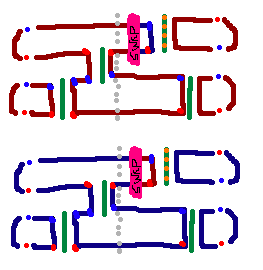
\includegraphics[width=2.4 in]{oplist.png} \caption{ 
\label{oplist} A possible VB-spin-operator diagram for a 4-site system with m=2 operators per copy of the system, {\bf (something about ratio and used to calculate the 2nd renyi entropy)
(also, make sure the two copies have *different* operators and loops, but still compatible spin configurations)}
}
} \end{figure}


\subsubsection{Flip...?}
\noindent 
{\bf
- keep the loops the same, flip all the spins.\\
- causes some diagonal operators to become off-diagonal and vice versa
}
\subsubsection{$\langle Swap_A \rangle$ measurement}
\noindent
{\bf 
- renyi measurement \\
- need to multiply by weight factor to get the actual measurement values\\
- energy (and other measurements) could be doubled (or alpha-ed) because we have multiple copies of the system
}
\subsubsection{Updating the operator list}
\noindent
{\bf- keep off-diagonal bond operators, move diagonal bond operators to a random, compatible spot.}
	
\subsection{Swap operator for $\alpha > 2$}

\begin{figure} {
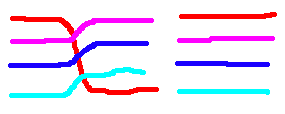
\includegraphics[width=2.4 in]{swap.png} \caption{ 
\label{swap_4} 
The cyclical permutation of states in region $A$ for four copies of a system.
}
} \end{figure}

\bibliography{}

\end{document}
